\documentclass[11pt]{report}

\usepackage[top= 1.5in, bottom= 1.5in]{geometry}
\usepackage{graphicx}
\usepackage{hyperref}
\usepackage{fancyvrb}
\usepackage{fancyhdr}

\pagestyle{fancy}\pagestyle{fancy}

\setlength{\textheight}{22.0cm}
\fancyfoot[C]{--- \thepage\ ---}
\renewcommand{\sectionmark}[1]{\markright{\thesection.\ #1}}

\fancypagestyle{plain}{\fancyhf{} 
                       \fancyfoot[C]{--- \thepage\ ---}
                       \renewcommand{\headrulewidth}{0pt}
                       \renewcommand{\footrulewidth}{0pt}
}



\begin{document}

\begin{center}

\includegraphics [scale=0.25] {GUClogo.pdf}
\\
\textbf{Faculty of Media Engineering and Technology}
\\
\textbf{German University in Cairo}
\\

\includegraphics [scale=0.75] {DHBWlogo.png}
\\
\textbf{Faculty of Computer Science}
\\
\textbf{Duale Hochschule Baden-Wurttemberg}
\vspace{2cm}
\\
\begin{huge}
\textbf{Static Program Analysis for \textsc{SetlX}}
\end{huge}
\\[2cm]
\textbf{Bachelor Thesis}
\begin{tabbing}\hspace{5cm}
Author: Ahmed AboulAzm\\\hspace{5cm}
Supervisor: Professor Karl Stroetmann\\\hspace{5cm}
Submission Date: {\today}
\end{tabbing}
\end{center}
\vspace{1.5cm}
I hereby certify that the thesis comprises only my original work towards my Bachelor Degree.
\begin{flushright}
\textbf{Ahmed AboulAzm}\\
\today
\end{flushright}

\pagebreak

\begin{center}
\begin{Large}
\underline{\textbf{ACKNOWLEDGMENT}}
\end{Large}
\end{center}

\vspace{2cm}

\begin{Large}
Foremost I would like to express my sincere gratitude to my advisor Prof. Karl Stroetmann for his continuous support in my bachelor project, for his patience, motivation, enthusiasm, and immense knowledge. His guidance helped me in all the time of implementation and writing this thesis. I could not have imagined having a better advisor and mentor for my bachelor project.\\

I would like also to thank my mother Amaal Morsi for her continuous support and encouragement, and for pushing me to do my bachelor project abroad. I wouldn't have made it without her.\\

I would also like to express my sincere thanks to Heidy Heweidy for her continuous support throughout my bachelor project.\\

Last but not least, I would like to thank my sister Deena Aboulazm and my friends for always being there for me when I needed support.
\end{Large}


\tableofcontents

\chapter{Introduction}
As \textsc{SetlX} is an untyped language, type errors are only caught at runtime.  This is the same
as in untyped languages like \textsl{Prolog} or \textsl{Python}.  However, current \textsl{Prolog}
implementations check for \emph{singleton variables}, i.e.~variables that are used only once.  The
reason is that many typos result in singleton variables.  Therefore, checking singleton variables
can uncover mistyped variable names.  Our intention 
is to implement similar static analysis techniques for \textsc{SetlX}.  In contrast to
\textsl{Prolog} programs, where a predicate can both read a variable and define it, the direction of
the data flow in \textsc{SetlX} programs is well defined.  Therefore, it is possible to implement a
static analysis for \textsc{SetlX} programs that is more precise than the corresponding analysis for
\textsl{Prolog}:  In particular, six main different checks are possible.

\begin{enumerate}
\item We can check whether a variable is defined before it is used.
      This is commonly referred to as definite assignment analysis.
\item We can check whether a variable is read after it is written.  If a variable is written but
      never read afterwards, the assignement to this variable is useless.  This kind of data flow
      analysis is known as live variable analysis.
\item Checking if any used procedure or class are defined in the code or not.
\item Checking that any procedure or class are called with the correct number of parameters.
\item Checking if all member variables and procedures called for objects actually do exist or not.
\item Giving a warning in classes in case the user defined a new variable with the same name of a class variable due to not adding a prefix \texttt{this.} before the variable's name.
\end{enumerate}

The following chapters are going to be as follows
\begin{enumerate}
\item Chapter 2 : is an introduction about the main language \textsc{setlX}.
\item Chapter 3 : discusses the implementation of the analyzer.
\item Chapter 4 : covers the part concerning regression tests.
\item Chapter 5 : is the conclusion of this thesis.
\end{enumerate}

\chapter{Introducing \textsc{setlX}}

\textsc{setlX} has been upgraded lately from the old untyped language \href{http://en.wikipedia.org/wiki/SETL}{\emph{SETL}}. It has been invented mainly for educational purposes as it is well suited to familiarize students with set theory, terms and functional programming.

In the following sections we are going to introduce the most important features of this language.

\begin{center} If you wish to see the official full tutorial and instructions to download \textsc{setlX} kindly visit this following link : 

\url{http://wwwlehre.dhbw-stuttgart.de/~stroetma/SetlX/setlX.php} \end{center}

\section{\textsc{SetlX} Data Types}

\textsc{setlX} is an interpreter that can be used to evaluate simple expressions. For example by typing 
\\[0.2cm]
\hspace*{1.3cm}
\texttt{\textsl{1/3 + 2/5;}}
\\[0.2cm]
and hitting return yields to this response
\\[0.2cm]
\hspace*{1.3cm}
\texttt{\symbol{126}< Result: 11/15 >\symbol{126}}
\\[0.2cm]
This example shows that \textsc{setlX} actually supports rational numbers, it also makes sure that the answer is in the simplest form. So after typing
\\[0.2cm]
\hspace*{1.3cm}
\texttt{\textsl{1/3 + 2/3;}}
\\[0.2cm]
The response would be
\\[0.2cm]
\hspace*{1.3cm}
\texttt{\symbol{126}< Result: 1 >\symbol{126}}
\\[0.2cm]
as in this case, the simplest form of the result will have a denominator of 1, thus \textsc{setlX} only prints the nominator.

The precision of any result computed in \textsc{setlX} is unlimited unless there is no more memory space to take it, so if we compute the factorial of 50
\\[0.2cm]
\hspace*{1.3cm}
\texttt{\textsl{50!;}}
\\[0.2cm]
The result would be
\\[0.2cm]
\hspace*{0.6cm}
\texttt{\symbol{126}< Result: 30414093201713378043612608166064768844377641568960512000000000000 >\symbol{126}}
\\[0.2cm]
To calculate floating point values in \textsc{setlX} the simplest way is to add 0.0 to the calculated expression as in
\\[0.2cm]
\hspace*{1.3cm}
\texttt{\textsl{1/3 + 2/5 + 0.0;}}
\\[0.2cm]
which will yield to a result in this case as shown
\\[0.2cm]
\hspace*{1.3cm}
\texttt{\symbol{126}< Result: 0.7333333333333333 >\symbol{126}}
\\[0.2cm] 

To create a string in \textsc{setlX}, you just need to put some characters between double quotations. Which makes the \textsl{hello world program} in \textsc{setlX}'s interactive mode as simple as
\\[0.2cm]
\hspace*{1.3cm}
\texttt{\textsl{\symbol{34}Hello world!\symbol{34};}}
\\[0.2cm]
which outputs 
\\[0.2cm]
\hspace*{1.3cm}
\texttt{\symbol{126}< Result: "Hello world!" >\symbol{126}}
\texttt{}
\\[0.2cm]

To assign a value to a variable in \textsc{setlX}, we use the ':=' operator which is the major difference between \textsc{setlX} and the programming language \textsl{C}
so writing 
\\[0.2cm]
\hspace*{1.3cm}
\texttt{\textsl{x := 2;}}
\\[0.2cm]
assigns the value '2' to the variable 'x'. Always keep in mind that in \textsc{setlX} variables always have to start with a lower case.
\\
\\
\textsc{setlX} provides some operators to combine boolean expressions. Which are
\begin{enumerate}
\item \texttt{\&\&} as the logical and.
\item \texttt{||} as the logical or.
\item \texttt{!} as the logical not.
\item \texttt{=>} as the logical implication.
\item \texttt{<==>} as the logical equivalence which can be also replaced with \texttt{==}.
\item \texttt{<!=>} as the logical antivalence which can be also replaced with \texttt{!=}.
\end{enumerate}
It provides some operators to create boolean expressions as well such as \texttt{>,<,==,!=,<=,>=}.


It also supports the universal and existential quantifiers \textsl{"forall"} and \textsl{"exists"}.
So in order to evaluate the formula
\\[0.2cm]
\hspace*{1.3cm}
$\forall x \in \{ 1, \cdots, 10 \}: x^2 \leq 2^x$
\\[0.2cm]
we simply write
\\[0.2cm]
\hspace*{1.3cm}
\texttt{forall (x in \{1..10\} | x ** 2 <= 2 ** x);}
\\[0.2cm]
and to evaluate
\\[0.2cm]
\hspace*{1.3cm}
$\exists x \in \{ 1, \cdots, 10 \}: 2^x < x^2$
\\[0.2cm]
we simply write
\\[0.2cm]
\hspace*{1.3cm}
\texttt{exists (x in \{1..10\} | 2 ** x < x ** 2);}
\\[0.2cm]
\\
The most interesting data type in \textsc{setlX} is the \textsl{set} type. You can create a \textsl{set} by writing
\\[0.2cm]
\hspace*{1.3cm}
\texttt{\{1, 2, 3\};}
\\[0.2cm]
which is exactly the same as writing
\\[0.2cm]
\hspace*{1.3cm}
\texttt{\{2, 1, 3\};}
\\[0.2cm]
as order doesn't matter in \textsl{sets}. \textsc{setlX} also provides other convenient ways of creating sets, for example writing
\\[0.2cm]
\hspace*{1.3cm}
\texttt{\{1..15\};}
\\[0.2cm]
will create a \textsl{set} containing all elements counting from 1 till 15 with a step of 1. While writing
\\[0.2cm]
\hspace*{1.3cm}
\texttt{\{a,b..c\};}
\\[0.2cm]
will create a \textsl{set} containing all elements counting from $a$ till $c$ with a step of $b-a$. The same also applies for descending orders.
\\
There are some basic operators on sets which are
\begin{enumerate}
\item \texttt{"+"} to compute the union of 2 sets.
\item \texttt{"*"} to compute the intersection of 2 sets.
\item \texttt{"-"} to compute the difference of 2 sets.
\item \texttt{"><"} to compute the cartesian product of 2 sets.
\item \texttt{"** 2"} to compute the cartesian product of a set with itself.
\item \texttt{"2 **"} to compute the power set of a set.
\item \texttt{"\%"} to compute the symmetric difference of 2 sets.
\end{enumerate}

Another interesting thing about \textsl{sets} in \textsc{setlX} is set comprehension which is used to build sets which has the general formula of
\\[0.2cm]
\hspace*{1.3cm}
\texttt{\{ $\textsl{expr}$ :$\;x_1$ in $s_1$, $\cdots$, $x_n$ in $s_n$ | $\textsl{cond}$ \}}.
\\[0.2cm]
where \textsl{expr} is an expression that contains $x_1$, $\cdots$, $x_n$ in it which are bound to the values inside $s_1$, $\cdots$, $s_n$ while \textsl{cond} is an extra optional condition if needed. For example 
\\[0.2cm]
\hspace*{1.3cm}
\texttt{\{ a * b : a in \{ 1 .. 3 \}, b in \{ 1 .. 3 \} \};}
\\[0.2cm]
computes the set
\\[0.2cm]
\hspace*{1.3cm}
\texttt{\{1, 2, 3, 4, 6, 9\}}.
\\[0.2cm]
This is actually very powerful, as by very simple code like
\\[0.2cm]
\hspace*{1.3cm}
\texttt{s := \{2..100\};}
\\
\hspace*{1.3cm}
\texttt{s - \{ p * q : p in s, q in s \};}
\\[0.2cm]
yields to an output containing all prime numbers between 1 and 100.
\textsc{setlX} also supports some set functions which make things easier like
\\[0.2cm]
\hspace*{1.3cm}
\texttt{first($s$)}
\\[0.2cm]
which returns the \emph{first} element of the set $s$, and
\\[0.2cm]
\hspace*{1.3cm}
\texttt{last($s$)} 
\\[0.2cm]
which returns the \emph{last} element of the set $s$.
\\
\\
\textsc{setlX} also supports lists which have 2 main differences with sets which are :
\begin{enumerate}
\item A syntactical difference : the
curly braces ``\texttt{\{}'' and ``\texttt{\}}'' of sets are substituted with the square brackets
``\texttt{[}'' and ``\texttt{]}'' for lists.
\item A logical difference :  A list is an ordered collection of elements which can contain an element more than once unlike sets.
\end{enumerate} 
Apart from these two points, lists are almost the same as sets and they support everything mentioned above concerning sets.
\\

Alike \textsc{setL} the old version of \textsc{setlX}, \textsc{setlX} pairs are supported. A pair is represented in \textsc{setlX} as a list of length two. A binary relation can be represented as a set of pairs. So if we can consider \textsl{r} as a binary relation, then we have a domain and a range represented in the formulas 
\\[0.2cm]
\hspace*{1.3cm}
\texttt{domain(r) = \{ x :[x,y] in r \}} \quad and \quad
\texttt{range(r)  = \{ y :[x,y] in r \}}.
\\[0.2cm]
Furthermore, binary relations can be used as a map. In that case if \textsl{r} is the binary relation, we have a definition for $r[x]$
\\[0.2cm]
\hspace*{1.3cm}
$r[x] := \left\{
\begin{array}{ll}
  y & \mbox{if the set $\{ y \mid [x,y] \in r\}$ contains exactly one element $y$;} \\[0.2cm]
  \Omega & \mbox{otherwise}.
\end{array} \right.
$
\\[0.2cm]
The symbol $\Omega$ in \textsc{setlX} appears when there is no solution or result to a certain expression.

Binary relations seem very helpful that they actually can be used as functions, but that won't be smart as that would consume a lot of memory and will compute even cases that aren't needed. Thus in \textsc{setlX} \textsl{procedures} are used for that. Figure \ref{fig:primes.stlx} for example defines a procedure that computes prime numbers starting $2$ up to a given number $n$.
\begin{figure}[!ht]
\centering
\begin{Verbatim}[ frame         = lines, 
                  framesep      = 0.3cm, 
                  firstnumber   = 1,
                  labelposition = bottomline,
                  numbers       = left,
                  numbersep     = -0.2cm,
                  xleftmargin   = 0.8cm,
                  xrightmargin  = 0.8cm,
                ]
    primes := procedure(n) { 
        s := { 2..n }; 
        return s - { p*q : p in s, q in s }; 
    };
\end{Verbatim}
\vspace*{-0.3cm}
\caption{A procedure to compute the prime numbers.}
\label{fig:primes.stlx}
\end{figure}

In Figure \ref{fig:primes.stlx}, the block starts with assigning ``\texttt{procedure(n) \{}'' to a variable \texttt{primes} which is the name of the procedure where $n$ in this case is the parameter given to this \textsl{procedure}, then the procedure's block ends with a closing bracket ``\texttt{\}}'' followed by a semi column \texttt{';'}. The procedure's block itself contains the logic that the procedure has to perform.\\
In \textsc{setlX} procedures can be
\begin{enumerate}
\item assigned to a variable.
\item used as an argument to another procedure.
\item be returned from other procedures.
\end{enumerate}
more about procedures will be discussed later on.
\\

Strings in \textsc{setlX} are a sequence of characters enclosed by double quotes. Here is a list of functions that can be applied to \textsl{Strings} in \textsc{setlX} :
\begin{enumerate}
\item \texttt{s1 + s2}: \texttt{+} to concatenate strings $s1$ and $s2$.
\item \texttt{s * n} : \texttt{*} to concatenate multiple instances of the string $s$ $n$ times where $n$ is a natural number.
\item \texttt{s[i]} : to get the $i_{th}$ character of string $s$.
\end{enumerate}
\textsc{setlX} also provides \textsl{string interpolation} where any string containing substring of it enclosed between two ``\texttt{\symbol{36}}'' signs, \textsc{setlX} evaluates the expression between them then substitute the result of it into the string. For example, if $n$ has the value of $6$
\\[0.2cm]
\hspace*{1.3cm}
\texttt{print(\symbol{34}\symbol{36}n\symbol{36}! = \symbol{36}n!\symbol{36}\symbol{34})};
\\[0.2cm]
will actually print
\\[0.2cm]
\hspace*{1.3cm}
\texttt{6! = 720}.
\\[0.2cm]
If you wish to turn off such kinds of processing, you just have to use single quotes instead of double quotes. For example
\\[0.2cm]
\hspace*{1.3cm}
\texttt{print('\symbol{36}n\symbol{36}! = \symbol{36}n!\symbol{36}')};
\\[0.2cm]
will actually print
\\[0.2cm]
\hspace*{1.3cm}
\texttt{\$n\$! = \$n!\$}.
\\[0.2cm]
\\

\textsc{setlX} provides also \textsl{first order terms} similar to the one provided by the programming language \textsl{Prolog}. Terms consists of \textsl{functors} and \textsl{arguments}. The difference between a \textsl{functor} and a \textsl{function} is that \textsl{functors} start with a capital letter and don't evaluate anything. An example for using \textsl{Terms} is implementing \href{http://en.wikipedia.org/wiki/Binary_search_tree}{\emph{ordered binary trees}}.
\begin{enumerate}
\item An empty tree is represented as
      \\[0.2cm]
      \hspace*{1.3cm}
      $\mathtt{Nil()}$
      \\[0.2cm]
\item A non-empty tree has three components
      \begin{enumerate}
      \item The \emph{root} node.
      \item A left subtree.
      \item A right subtree.
      \end{enumerate}
represented as 
	  \\[0.2cm]
      \hspace*{1.3cm}
      $\texttt{Node}(k, l, r)$,
      \\[0.2cm]
where $k$ is the element stored at the root, $l$ is the left subtree and $r$ is the right subtree. For example the term
\\[0.2cm]
\hspace*{1.3cm}
\texttt{Node(2,Node(1,Nil(),Nil), Node(3,Nil(), Nil()))}
\\[0.2cm]
is actually representing the tree that looks as follows
\begin{center} 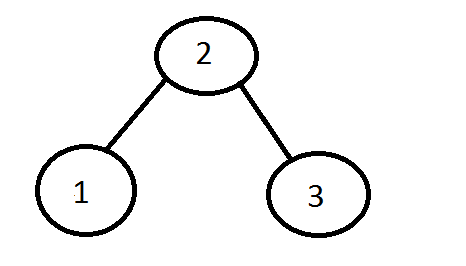
\includegraphics[width=1.5in, height=1.5in, scale=1, angle=0]{binary-tree.png} \end{center}
\end{enumerate}
\textsc{setlX} supports 3 main functions for terms.
\begin{enumerate}
\item \texttt{fct(t)} which returns the functor of a term $t$.
\item \texttt{args(t)} which returns the arguments of a term $t$.
\item \texttt{makeTerm(f,l)} which creates a term of functor $f$ and arguments $l$.
\end{enumerate}
So executing \texttt{fct(Node(3,Nil(),Nil()))} yields a result of \texttt{"Node"},\\
and executing \texttt{args(Node(3,Nil(),Nil()))} yields a result of \texttt{[3, Nil(), Nil()]},\\
and executing \texttt{makeTerm(\symbol{34}Node\symbol{34},[ makeTerm(\symbol{34}Nil\symbol{34},[]), makeTerm(\symbol{34}Nil\symbol{34},[]) ])} constructs the term \texttt{Node(3, Nil(), Nil())}.
\\
\\
Figure \ref{fig:binary-tree-no-matching.stlx} actually shows how terms can be used in \textsc{setlX} to implement ordered binary trees.
\pagebreak
\begin{figure}[!ht]
\centering
\begin{Verbatim}[ frame         = lines, 
                  framesep      = 0.3cm, 
                  firstnumber   = 1,
                  labelposition = bottomline,
                  numbers       = left,
                  numbersep     = -0.2cm,
                  xleftmargin   = 0.8cm,
                  xrightmargin  = 0.8cm,
                ]
    insert := procedure(m, k1) {
        switch {
            case fct(m) == "Nil" : 
                 return Node(k1, Nil(), Nil());
            case fct(m) == "Node": 
                 [ k2, l, r ] := args(m);
                 if (k1 == k2) {
                     return Node(k1, l, r);
                 } else if (compare(k1, k2) < 0) { 
                     return Node(k2, insert(l, k1), r);
                 } else {
                     return Node(k2, l, insert(r, k1));
                 }
        }
    };
\end{Verbatim}
\vspace*{-0.3cm}
\caption{Inserting an element into a binary tree.}
\label{fig:binary-tree-no-matching.stlx}
\end{figure}

In an ordered binary tree any node will have nodes with lower values inserted on left of it and any nodes with higher values inserted on right of it, and in case the inserted node has the same value of an existing node then it won't be inserted into the tree. This is exactly what happens in the example shown in Figure \ref{fig:binary-tree-no-matching.stlx} where $m$ represents the tree and $k1$ represents the value of the node to be inserted. The tree's parent node is first checked if it's empty by checking if the functor of this node is \texttt{Nil} which will match the first case of the switch statement. If that condition is true then the returned tree will just be the newly inserted node, otherwise if it's a non-empty \texttt{Node} it will then match the second statement, in this case at line '$6$' $k2$ will have the value of this node while $l$ and $r$ will hold the left and right sub-trees of this node respectively. After that three nested \textsl{if-conditions} are executed. If the inserted node's value has the same value of the current node being checked then it just returns the original tree $m$, otherwise if it has a lower value then a recursion happens only this time checking the inserted node with the left sub-tree, the same goes for the case if the inserted node is higher only this time with the right sub-tree. 

\section{Statements in \textsc{setlX}}
In this section we are going to talk about different kinds of statements in \textsc{setlX}. The most basic statements are the assignment statements. In \textsc{setlX}, you can have a single assignment like
\\[0.2cm]
\hspace*{1.3cm}
\texttt{x := 2;}
\\[0.2cm]
which assigns the variable $x$ to the value of $2$. Chained assignments can also be used as
\\[0.2cm]
\hspace*{1.3cm}
\texttt{a := b := 2;}
\\[0.2cm]
which assigns both variables $a$ and $b$ to the value of 2, you can also have simultaneous assignments at the same time like
\\[0.2cm]
\hspace*{1.3cm}
\texttt{[x, y, z] := [1, 2, 3];}
\\[0.2cm]
which assigns variable $x$ to a value of 1, variable $y$ to a value of 2 and variable $z$ to a value of 3. Simultaneous assignment can also be useful when swapping values is needed. For example, the statement
\\[0.2cm]
\hspace*{1.3cm}
\texttt{[x, y] := [y, x];}
\\[0.2cm]
actually swaps the values between $x$ and $y$.
\\

Functions and their structure have been discussed before but lets see some more examples about them. Looking at Figure \ref{fig:primes-slim.stlx}, the first function 'factors' is a function that computes the factors of a given number while the second one 'primes' make use of the function 'factors' to compute all prime numbers upto a given number $p$. We can give a grammar rule for defining a function as
\\[0.2cm]
\hspace*{1.3cm}
\texttt{fctDef -> VAR ":=" "procedure" "(" paramList ")" "{" block "}" ";"}
\\[0.2cm]
where the symbols in this grammar means the following
\begin{enumerate}
\item \texttt{VAR} is a variable which will be used as the name of the function further on.
\item \texttt{paramList} is the list of parameters used in the function separated by commas. Parameters can just be a variable name or a variable name preceded by "rw" which means that this variable is a "read-write" variable and after the procedure is executed, that variable's value might actually be changed.
\item \texttt{block} is the code holding the logic of the function itself.
\end{enumerate}

\begin{figure}[!ht]
\centering
\begin{Verbatim}[ frame         = lines, 
                  framesep      = 0.3cm, 
                  firstnumber   = 1,
                  labelposition = bottomline,
                  numbers       = left,
                  numbersep     = -0.2cm,
                  xleftmargin   = 0.8cm,
                  xrightmargin  = 0.8cm,
                ]
    factors := procedure(p) {
        return { f in { 1 .. p } | p % f == 0 };
    };
    primes := procedure(n) {
        return { p in { 2 .. n } | factors(p) == { 1, p } };
    };
    print(primes(100));
\end{Verbatim}
\vspace*{-0.3cm}
\caption{A naive program to compute primes.}
\label{fig:primes-slim.stlx}
\end{figure}

There is actually a simpler way to define a procedure in \textsc{setlX} if the procedure's logic is a single expression, which is called the lambda definition and has the grammar rule
\\[0.2cm]
\hspace*{1.3cm}
\texttt{fctDef -> ID ":=" "lambdaParams" "|->" exp ";"}
\\[0.2cm]
where \texttt{lambdaParams} is either a single parameter or a set of parameters enclosed by square brackets. An example of using the lambda definition is
\\[0.2cm]
\hspace*{1.3cm}
\texttt{double := x |-> x*2;}
\\[0.2cm]
\\

\textsc{setlX} supports \textsl{if-then-else statements}, \textsl{switch statements} and \textsl{match statements}. An example of the use of the \textsl{if-then-else statements} is shown in Figure \ref{fig:toBin.stlx} while an example for the use of the \textsl{switch statements} is shown in Figure \ref{fig:sort3.stlx}.

\begin{figure}[!ht]
\centering
\begin{Verbatim}[ frame         = lines, 
                  framesep      = 0.3cm, 
                  firstnumber   = 1,
                  labelposition = bottomline,
                  numbers       = left,
                  numbersep     = -0.2cm,
                  xleftmargin   = 0.8cm,
                  xrightmargin  = 0.8cm,
                ]
    toBin := procedure(n) {
        if (n < 2) {
            return str(n);
        } else {
            r := n % 2;
            n := floor(n / 2);
            return toBin(n) + toBin(r);
        }
    };
\end{Verbatim}
\vspace*{-0.3cm}
\caption{A function to compute the binary representation of a natural number.}
\label{fig:toBin.stlx}
\end{figure}

\begin{figure}[!ht]
\centering
\begin{Verbatim}[ frame         = lines, 
                  framesep      = 0.3cm, 
                  firstnumber   = 1,
                  labelposition = bottomline,
                  numbers       = left,
                  numbersep     = -0.2cm,
                  xleftmargin   = 0.8cm,
                  xrightmargin  = 0.8cm,
                ]
    sort3 := procedure(l) {
        [ x, y, z ] := l;
        if (x <= y) {
            if (y <= z) {
                return [ x, y, z ];
            } else if (x <= z) { 
                return [ x, z, y ];
            } else {
                return [ z, x, y ];
            }
        } else if (z <= y) { 
            return [z, y, x];
        } else if (x <= z) { 
            return [ y, x, z ];
        } else {
            return [ y, z, x ];
        }
    };
\end{Verbatim}
\vspace*{-0.3cm}
\caption{A function to sort a list of three elements.}
\label{fig:sort3.stlx}
\end{figure}

As for match statements, there are different types of matching statements. One kind is called \textsl{string-matching}. One example for it is shown in Figure \ref{fig:reverse.stlx}

\begin{figure}[!ht]
\centering
\begin{Verbatim}[ frame         = lines, 
                  framesep      = 0.3cm, 
                  firstnumber   = 1,
                  labelposition = bottomline,
                  numbers       = left,
                  numbersep     = -0.2cm,
                  xleftmargin   = 0.8cm,
                  xrightmargin  = 0.8cm,
                ]
    reverse := procedure(s) {
        match (s) {
            case []   : return s;
            case [c|r]: return reverse(r) + c;
            default   : abort("type error in reverse($s$)");
        }
    };
\end{Verbatim}
\vspace*{-0.3cm}
\caption{A function that reverses a string.}
\label{fig:reverse.stlx}
\end{figure}
Calling \texttt{reverse("abc");} will yield an output of "cba". There are other kinds of matching like \textsl{list-matching}, \textsl{set-matching} and \textsl{term-matching}. Term-Matching is the most elaborate form of matching, it's similar to the matching provided in programming languages \href{http://en.wikipedia.org/wiki/Prolog}{\textsl{Prolog}} and 
\href{http://en.wikipedia.org/wiki/ML_(programming_language)}{\textsc{Ml}}. An example for \textsl{term-matching} is shown in Figure \ref{fig:binary-tree.stlx} which does the same work as the code shown in Figure \ref{fig:binary-tree-no-matching.stlx} discussed previously.

\begin{figure}[!ht]
\centering
\begin{Verbatim}[ frame         = lines, 
                  framesep      = 0.3cm, 
                  firstnumber   = 1,
                  labelposition = bottomline,
                  numbers       = left,
                  numbersep     = -0.2cm,
                  xleftmargin   = 0.8cm,
                  xrightmargin  = 0.8cm,
                ]
    insert := procedure(m, k1) {
        match (m) {
            case Nil() : 
                 return Node(k1, Nil(), Nil());
            case Node(k2, l, r): 
                 if (k1 == k2) {
                     return Node(k1, l, r);
                 } else if (compare(k1, k2) < 0) { 
                     return Node(k2, insert(l, k1), r);
                 } else {
                     return Node(k2, l, insert(r, k1));
                 }
            default: abort("Error in insert($m$, $k1$, $v1$)");
        }
    };
\end{Verbatim}
\vspace*{-0.3cm}
\caption{Inserting an element into a binary tree using matching.}
\label{fig:binary-tree.stlx}
\end{figure}

A more complex example is shown in Figure \ref{fig:diff.stlx} which computes the derivative of $t$ relative to $x$. In order to understand this example better, we have to discuss some predefined functions which convert strings to terms which are the \textsl{canonical} and the \textsl{parse} functions. These functions are going to be discussed in the last section entitled \textsl{predefined functions}.

\begin{figure}[!ht]
\centering
\begin{Verbatim}[ frame         = lines, 
                  framesep      = 0.3cm, 
                  firstnumber   = 1,
                  labelposition = bottomline,
                  numbers       = left,
                  numbersep     = -0.2cm,
                  xleftmargin   = 0.8cm,
                  xrightmargin  = 0.8cm,
                ]
    diff := procedure(t, x) {
        match (t) {
            case t1 + t2 :
                return diff(t1, x) + diff(t2, x);
            case t1 - t2 :
                return diff(t1, x) - diff(t2, x);
            case t1 * t2 :
                return diff(t1, x) * t2 + t1 * diff(t2, x);
            case t1 / t2 :
                return ( diff(t1, x) * t2 - t1 * diff(t2, x) ) / t2 * t2;
            case f ** g :
                return diff( @exp(g * @ln(f)), x);
            case ln(a) :
                return diff(a, x) / a;
            case exp(a) :
                return diff(a, x) * @exp(a);
            case ^variable(x) : // x is defined above as second argument
                return 1;
            case ^variable(y) : // y is undefined, matches any other variable
                return 0;
            case n | isNumber(n):   
                return 0;  
        }
    };
\end{Verbatim}
\vspace*{-0.3cm}
\caption{A function to perform symbolic differentiation.}
\label{fig:diff.stlx}
\end{figure}

\textsc{setlX} offers two kinds of loops which are the \textsl{while loops} and the \textsl{for loops}. The while loops follows the grammar rule
\\[0.2cm]
\hspace*{1.3cm}
\texttt{statement -> "while" "(" boolExpr ")" "{" block "}" }.
\\[0.2cm]
Figure \ref{fig:ulam.stlx} is an example for implementing \href{http://en.wikipedia.org/wiki/Collatz_conjecture}{\emph{Collatz conjecture}}: which is represented as the recursive function $f$ with definition
\begin{enumerate}
\item $f(n) := 1$ \hspace*{2.13cm} if $n \leq 1$,
\item $f(n) := \left\{
       \begin{array}[c]{ll}
         f(n/2)           & \mbox{if $n \,\texttt{\symbol{37}}\, 2 = 0$;} \\[0.2cm]  
         f(3 \cdot n + 1) & \mbox{otherwise.} 
       \end{array}
       \right.
      $ 
\end{enumerate}
using the while loop.
\begin{figure}[!ht]
\centering
\begin{Verbatim}[ frame         = lines, 
                  framesep      = 0.3cm, 
                  firstnumber   = 1,
                  labelposition = bottomline,
                  numbers       = left,
                  numbersep     = -0.2cm,
                  xleftmargin   = 0.8cm,
                  xrightmargin  = 0.8cm,
                ]
    f := procedure(n) {
        if (n == 0) {
            return 1;   
        }
        while (n != 1) {
            if (n % 2 == 0) {
                n /= 2;
            } else {
                n := 3 * n + 1;
            }
        }
        return n;
    };
\end{Verbatim}
\vspace*{-0.3cm}
\caption{A program to test the Collatz conjecture.}
\label{fig:ulam.stlx}
\end{figure}

On the other hand \textsl{for-loops} follow the grammar rule
\\[0.2cm]
\hspace*{1.3cm}
\texttt{statement -> "for" "(" iterator("," iterator)* ")" "{" block "}" }.
\\[0.2cm]
A simple iterator would be $x$ in $s$ where $s$ is a set or a list or a string. An example for the usage of \textsl{for-loops} is represented in Figure \ref{fig:multiplication-table.stlx} and has an output represented in Figure \ref{fig:multiplication-table}.
\begin{figure}[!ht]
\centering
\begin{Verbatim}[ frame         = lines, 
                  framesep      = 0.3cm, 
                  firstnumber   = 1,
                  labelposition = bottomline,
                  numbers       = left,
                  numbersep     = -0.2cm,
                  xleftmargin   = 0.8cm,
                  xrightmargin  = 0.8cm,
                ]
    rightAdjust := procedure(n) {
        switch {
            case n < 10 : return "   " + n;
            case n < 100: return  "  " + n;
            default:      return   " " + n;
        }
    };      
    for (i in [1 .. 10]) {
        for (j in [1 .. 10]) {
            nPrint(rightAdjust(i * j));
        }
        print();
    }
\end{Verbatim}
\vspace*{-0.3cm}
\caption{A simple program to generate a multiplication table.}
\label{fig:multiplication-table.stlx}
\end{figure}

\begin{figure}[!ht]
\centering
\begin{Verbatim}[ frame         = lines, 
                  framesep      = 0.3cm, 
                  firstnumber   = 1,
                  labelposition = bottomline,
                  numbers       = none,
                  numbersep     = -0.2cm,
                  xleftmargin   = 0.8cm,
                  xrightmargin  = 0.8cm,
                ]
       1   2   3   4   5   6   7   8   9  10
       2   4   6   8  10  12  14  16  18  20
       3   6   9  12  15  18  21  24  27  30
       4   8  12  16  20  24  28  32  36  40
       5  10  15  20  25  30  35  40  45  50
       6  12  18  24  30  36  42  48  54  60
       7  14  21  28  35  42  49  56  63  70
       8  16  24  32  40  48  56  64  72  80
       9  18  27  36  45  54  63  72  81  90
      10  20  30  40  50  60  70  80  90 100
\end{Verbatim}
\vspace*{-0.3cm}
\caption{Output of the program in Figure \ref{fig:multiplication-table.stlx}.}
\label{fig:multiplication-table}
\end{figure}
\pagebreak

\section{Regular Expressions}
\textsc{setlX} like most modern programming languages supports \href{http://en.wikipedia.org/wiki/Regular_expression}{\emph{Regular expressions}} which is a very powerful tool to process strings. Regular Expressions can be used in match statements. One example for that is shown in Figure \ref{fig:regexp.stlx} which is a procedure that takes a string and recognizes if it's a word, integer or just a white space.

\begin{figure}[!ht]
\centering
\begin{Verbatim}[ frame         = lines, 
                  framesep      = 0.3cm, 
                  firstnumber   = 1,
                  labelposition = bottomline,
                  numbers       = left,
                  numbersep     = -0.2cm,
                  xleftmargin   = 0.8cm,
                  xrightmargin  = 0.8cm,
                ]
    classify := procedure(s) {
        match (s) {
            regex '0|[1-9][0-9]*': print("found an integer");
            regex '[a-zA-Z]+'    : print("found a word");
            regex '\s+'          : // skip white space
            default              : print("unkown: $s$");
        }
    };
\end{Verbatim}
\vspace*{-0.3cm}
\caption{A simple function to recognize numbers and words.}
\label{fig:regexp.stlx}
\end{figure} 
Regular expressions also can be used for extracting substrings. Consider the example given in Figure \ref{fig:extract-phone-code.stlx} which extracts parts of a phone-code in the format of \texttt{+49-711-6673-4504} where $49$ is the country code, $711$ is the area code, $6673$ is the company code and $4504$ is the extension. In this example if an expression is matched, variable $c$ will have the country code, variable $a$ will have the area code, variable $co$ will have the company code, variable $x$ will have the extension, finally variable $e$ will hold the string that matched the whole regular expression.

\begin{figure}[!ht]
\centering
\begin{Verbatim}[ frame         = lines, 
                  framesep      = 0.3cm, 
                  firstnumber   = 1,
                  labelposition = bottomline,
                  numbers       = left,
                  numbersep     = -0.2cm,
                  xleftmargin   = 0.3cm,
                  xrightmargin  = 0.3cm,
                ]
    extractCountryArea := procedure(phone) {
        match (phone) {
            regex '\+([0-9]+)-([0-9]+)-([0-9]+)-([0-9]+)' as [e, c, a, co, x]:
                return [c, a];
            default: abort("The string $phone$ is not a phone number!");
        }
    };
\end{Verbatim}
\vspace*{-0.3cm}
\caption{A function to extract the country and area code of a phone number.}
\label{fig:extract-phone-code.stlx}
\end{figure}
\pagebreak
Regular expressions can also be used with \textsl{scan-statements} as shown in Figure \ref{fig:find-comments-scan.stlx}. \textsl{Scan statements} have the general form of
\\[0.2cm]
\hspace*{1.3cm} \texttt{scan ($s$) \{}  \\
\hspace*{1.8cm} \texttt{regex} $r_1$ \texttt{as} $l$ : $b_1$ \\
\hspace*{1.8cm} $\vdots$                                                  \\
\hspace*{1.8cm} \texttt{regex} $r_n$ \texttt{as} $l$ : $b_n$ \\
\hspace*{1.3cm} \texttt{\}}             
\\[0.2cm]

\begin{figure}[!ht]
\centering
\begin{Verbatim}[ frame         = lines, 
                  framesep      = 0.3cm, 
                  firstnumber   = 1,
                  labelposition = bottomline,
                  numbers       = left,
                  numbersep     = -0.2cm,
                  xleftmargin   = 0.8cm,
                  xrightmargin  = 0.8cm,
                ]
    printComments := procedure(file) {
        s := join(readFile(file), "\n");
        scan (s) {
            regex '//[^\n]*'                as c: print(c[1]);
            regex '/\*([^*]|\*+[^*/])*\*+/' as c: print(c[1]);
            regex '.|\n'                        : // skip every thing else
        }
    };
\end{Verbatim}
\vspace*{-0.3cm}
\caption{Extracting comments using the match statement.}
\label{fig:find-comments-scan.stlx}
\end{figure}

Given bellow are some examples for predefined functions for regular expressions.
\begin{enumerate}
\item \texttt{testRegexp('(a*)(a+)b',"aaab");} yields a result \texttt{["aaab", "aa", "a"]} where every item of the list is defined by the order of the opening parenthesis.
\item \texttt{matches('(a*)(a+)b',"aaab", true);} with three arguments with the last one defined as a boolean \textsl{true} has the exact same effect as the \texttt{testRegexp} and has the same return value of \texttt{["aaab", "aa", "a"]}.
\item \texttt{matches('(a*)(a+)b',"aaab");} with two arguments returns true if the string given matches the regular expression or false otherwise. In this case given in the example the result would be true.
\item \texttt{replace(s, r, t)} replaces every substring of $s$ that matches the regular expression $r$ by the string $t$.
\end{enumerate}


\section{Functional Programming}
It has been stated previously that \textsc{setlX} is a full-fledged functional language. Functions can be used as arguments to other functions and as return values. There is no big difference between the type of a function and any other type that can be assigned to a variable.

Using functions as arguments to other functions is not that commonly seen in conventional programming languages. Figure \ref{fig:reduce.stlx} shows an example for that. In this example the function \textsl{reduce} takes two arguments which are $l$ as a list and $f$ as a function. What this function do is that it reduces the list to one single value at the end by combining all its elements by the function $f$, so if we could say that $f$ was an add function then the function \textsl{reduce} computes the sum of all its elements. In case the list was empty then the function returns the value om($\Omega$).

\begin{figure}[!ht]
\centering
\begin{Verbatim}[ frame         = lines, 
                  framesep      = 0.3cm, 
                  firstnumber   = 1,
                  labelposition = bottomline,
                  numbers       = left,
                  numbersep     = -0.2cm,
                  xleftmargin   = 0.8cm,
                  xrightmargin  = 0.8cm,
                ]
    reduce := procedure(l, f) {
        match (l) {
            case []     : return;
            case [x]    : return x;
            case [x,y|r]: return reduce([f(x,y) | r], f);
        }    
    };
    add      := procedure(a, b) { return a + b; };
    multiply := procedure(a, b) { return a * b; };
    
    l := [1 .. 36];
    x := reduce(l, add     );
    y := reduce(l, multiply);
\end{Verbatim}
\vspace*{-0.3cm}
\caption{Implementing a second order function.}
\label{fig:reduce.stlx}
\end{figure}

Another example for second order functions is shown in Figure \ref{fig:merge-sort.stlx}.

\begin{figure}[!ht]
\centering
\begin{Verbatim}[ frame         = lines, 
                  framesep      = 0.3cm, 
                  firstnumber   = 1,
                  labelposition = bottomline,
                  numbers       = left,
                  numbersep     = -0.2cm,
                  xleftmargin   = 0.8cm,
                  xrightmargin  = 0.8cm,
                ]
    sort := procedure(l, cmp) {
        if (#l < 2) { return l; }
        m := #l \ 2;
        [l1, l2] := [l[.. m], l[m+1 ..]];
        [s1, s2] := [sort(l1, cmp), sort(l2, cmp)];
        return merge(s1, s2, cmp);
    };
    merge := procedure(l1, l2, cmp) {
        match ([l1, l2]) {
            case [[], _] : return l2;
            case [_, []] : return l1;
            case [[x1|r1], [x2|r2]] : 
                 if (cmp(x1, x2)) {
                     return [x1 | merge(r1, l2, cmp)];
                 } else {
                     return [x2 | merge(l1, r2, cmp)];
                 }
        }
    };
    less    := procedure(x, y) { return x < y; };
    greater := procedure(x, y) { return y < x; };
    l  := [1,3,5,4,2];    
    s1 := sort(l, less   );
    s2 := sort(l, greater);
\end{Verbatim}
\vspace*{-0.3cm}
\caption{A generic sort function.}
\label{fig:merge-sort.stlx}
\end{figure}

In this example the function \textsl{sort} takes two arguments. The first argument $l$ is a list and the second argument $cmp$ is a function that compares two list elements and returns either true or false. What this function does is that it orders the list according to the second order function given as an argument. If for example the function \texttt{less} defined in line 20 was given as an argument, then the resulting list would be ordered ascendingly. If instead the function \texttt{greater} was the argument given, then the resulting list would be ordered descendingly.
\\

The previous two examples showed how functions can be used as arguments to other functions. As mentioned before functions can also be used as return values from other functions. Shown in Figure \ref{fig:finite-difference.stlx} is an example that computes the \textsl{discrete-derivative} of a certain function $f$. This example shows how functions can actually be used as a return value from other functions.

\begin{figure}[!ht]
\centering
\begin{Verbatim}[ frame         = lines, 
                  framesep      = 0.3cm, 
                  firstnumber   = 1,
                  labelposition = bottomline,
                  numbers       = left,
                  numbersep     = -0.2cm,
                  xleftmargin   = 0.8cm,
                  xrightmargin  = 0.8cm,
                ]
    delta := procedure(f) {
        return n |-> f(n+1) - f(n);
    };    
    g := n |-> n;
    h := n |-> 2 ** n;
    deltaG := delta(g);
    deltaH := delta(h);
    
    print([ deltaG(n) : n in [1 .. 10]]);
    print([ deltaH(n) : n in [1 .. 10]]);
\end{Verbatim}
\vspace*{-0.3cm}
\caption{Computing the discrete derivative of a given function.}
\label{fig:finite-difference.stlx}
\end{figure}
\pagebreak

\section{Exceptions and Backtracking}

\textsc{setlX} supports means of exception handling and backtracking. But since they are irrelevant to the project itself it won't be discussed here. To know more about them kindly check the official tutorial referenced at the beginning of this chapter. 

\section{Objects and Classes}
\textsc{setlX} supports some basic means of \href{http://en.wikipedia.org/wiki/Object-oriented_programming}{\emph{object-oriented programming}} most importantly classes. A \href{http://en.wikipedia.org/wiki/Class_(computer_programming)}{\emph{class}} is a collection of \textsl{member-variables} and \textsl{methods} where \textsl{member-variables} are some defined variables and the \textsl{methods} are some defined functions. Figure \ref{fig:point.stlx} shows an example for creating a class \textsl{point} which represents a point in a plane.

\begin{figure}[!ht]
\centering
\begin{Verbatim}[ frame         = lines, 
                  framesep      = 0.3cm, 
                  firstnumber   = 1,
                  labelposition = bottomline,
                  numbers       = left,
                  numbersep     = -0.2cm,
                  xleftmargin   = 0.8cm,
                  xrightmargin  = 0.8cm,
                ]
    class point(x, y) {
        mX := x;
        mY := y;
    
        getX  := procedure()  { return mX;             };
        getY  := procedure()  { return mY;             };
        setX  := procedure(x) { this.mX := x;          };
        setY  := procedure(y) { this.mY := y;          };
        toStr := procedure()  { return "<$mX$, $mY$>"; };

        distance := procedure(p) {
            return sqrt((mX - p.getX()) ** 2 + (mY - p.getY()) ** 2);
        };
    }
\end{Verbatim}
\vspace*{-0.3cm}
\caption{The class \texttt{point}.}
\label{fig:point.stlx}
\end{figure}

The first line of this example defines the class along with the constructor of this class where the constructor takes two arguments $x$ and $y$. The general form of a class definition is as follows

\vspace{0.2cm}
\hspace*{0.8cm}
\texttt{class} \textsl{name}$(x_1, \cdots, x_n)$ \texttt{\{}  
\\
\hspace*{2.0cm} \textsl{member-and-method-definitions}
\\
\hspace*{1.3cm}
\texttt{\}}
\\[0.2cm]
where \textsl{name} is the name of the class, $x_1, \cdots, x_n$ are the formal parameters of the constructor and \textsl{member-and-method-definitions} are the definitions of member variables and methods. In this example \textsl{mX and mY} are the defined member variables while \textsl{getX, getY, setX, setY, toStr and distance} are the class methods.

We can define an object \textsl{origin} of this class
\texttt{point} by writing
\\[0.2cm]
\hspace*{1.3cm}
\texttt{origin := point(0, 0);}
\\[0.2cm]
then if we would print the object itself by writing 
\\[0.2cm]
\hspace*{1.3cm}
\texttt{print(origin);}
\\[0.2cm]
that would yield the output shown in Figure \ref{fig:print_origin}. This output has been formatted this way to make it readable. Note that the constructor of the class \texttt{point} is part of the object origin.

\begin{figure}[!ht]
\centering
\begin{Verbatim}[ frame         = lines, 
                  framesep      = 0.3cm, 
                  firstnumber   = 1,
                  labelposition = bottomline,
                  numbers       = left,
                  numbersep     = -0.2cm,
                  xleftmargin   = 0.0cm,
                  xrightmargin  = 0.0cm,
                ]
    object<
        { distance := procedure(p) { 
                          return sqrt((mX-p.getX()) ** 2 + (mY-p.getY()) ** 2); 
                      }; 
          toStr := procedure() { return "<$mX$, $mY$>"; }; 
          setX  := procedure(x) { this.mX := x; }; 
          getY  := procedure() { return mY; }; 
          mX    := 0; 
          setY  := procedure(y) { this.mY := y; }; 
          getX  := procedure()  { return mX; }; 
          mY    := 0; 
          class (x, y) { 
              mX := x; 
              mY := y; 
              distance := procedure(p) { 
                  return sqrt((mX - p.getX()) ** 2 + (mY - p.getY()) ** 2); 
              }; 
              getX := procedure() { return mX; };
              getY := procedure() { return mY; }; 
              setX := procedure(x) { this.mX := x; }; 
              setY := procedure(y) { this.mY := y; }; 
              toStr := procedure() { return "<$mX$, $mY$>"; }; 
          } 
        }
    >
\end{Verbatim}
\vspace*{-0.3cm}
\caption{The output of the command ``\texttt{print(origin);}''.}
\label{fig:print_origin}
\end{figure}

The fact that all methods are stored as part of the object may seem redundant but in fact it's useful in case we needed to disable a method of the class from being used for a certain object. For example to disable the setter methods for the object \textsl{origin} by simply writing
\\[0.2cm]
\hspace*{1.3cm}
\texttt{origin.setX := om;}
\\
\hspace*{1.3cm}
\texttt{origin.setY := om;}
\\[0.2cm]

If we don't want to change methods on a per-object basis, we just need to declare these methods to be static as shown in Figure \ref{fig:point-static.stlx}.

\begin{figure}[!htb]
\centering
\begin{Verbatim}[ frame         = lines, 
                  framesep      = 0.3cm, 
                  firstnumber   = 1,
                  labelposition = bottomline,
                  numbers       = left,
                  numbersep     = -0.2cm,
                  xleftmargin   = 0.8cm,
                  xrightmargin  = 0.8cm,
                ]
    class point(x, y) {
        mX := x;
        mY := y;
    
      static {
        getX  := procedure()  { return mX;             };
        getY  := procedure()  { return mY;             };
        setX  := procedure(x) { this.mX := x;          };
        setY  := procedure(y) { this.mY := y;          };
        toStr := procedure()  { return "<$mX$, $mY$>"; };
 
        distance := procedure(p) {
            return sqrt((mX - p.getX()) ** 2 + (mY - p.getY()) ** 2);
        };
      }
    }
\end{Verbatim}
\vspace*{-0.3cm}
\caption{The class \texttt{point} implemented using static methods.}
\label{fig:point-static.stlx}
\end{figure}

Now in this case the command 
\\[0.2cm]
\hspace*{1.3cm}
\texttt{print(origin);}
\\[0.2cm]
will yield the output shown in Figure \ref{fig:point-static.stlx-origin}.

\begin{figure}[!ht]
\centering
\begin{Verbatim}[ frame         = lines, 
                  framesep      = 0.3cm, 
                  firstnumber   = 1,
                  labelposition = bottomline,
                  numbers       = left,
                  numbersep     = -0.2cm,
                  xleftmargin   = 0.0cm,
                  xrightmargin  = 0.0cm,
                ]
    object<
        { mX := 0; 
          mY := 0; 
          class (x, y) { 
              mX := x; 
              mY := y; 
            static { 
              distance := procedure(p) { 
                              return sqrt((mX-p.getX()) ** 2 + (mY-p.getY()) ** 2); 
                          }; 
              getX  := procedure()  { return mX;             }; 
              getY  := procedure()  { return mY;             }; 
              setX  := procedure(x) { this.mX := x;          }; 
              setY  := procedure(y) { this.mY := y;          }; 
              toStr := procedure()  { return "<$mX$, $mY$>"; }; 
            } 
          } 
        }
    >
\end{Verbatim}
\vspace*{-0.3cm}
\caption{Output of ``\texttt{print(origin);}''.}
\label{fig:point-static.stlx-origin}
\end{figure}

\section{Predefined Functions}

\textsc{setlX} provides a lot of predefined functions for
\begin{enumerate}
\item dealing with sets and strings.
\item dealing with strings.
\item working with terms.
\item working with mathematical functions.
\item dealing with objects.
\item supporting interactive debugging.
\item dealing with I/O.
\end{enumerate}

Some of the predefined functions have been mentioned earlier. Since there are too many predefined functions, we are only going to discuss the most important of them that are used in the implementation of the static analysis.

\begin{enumerate}
\item \texttt{+}: computes the union of its arguments which are either sets or lists.
\item \texttt{first}: The function $\texttt{first}(s)$ picks the first  element from the
      sequence $s$.  The argument $s$ can either be a set, a list, or a string.
      \item \texttt{fromB}: The function $\texttt{fromB}(s)$ picks the first element from the
      sequence $s$.  The argument $s$ can either be a set, a list, or a string.  This
      element is 
      removed from $s$ and returned.  This function returns the same element as the
      function \texttt{first} discussed previously.
\item \texttt{fromE}: The function $\texttt{fromB}(s)$ picks the last element from the
      sequence $s$.  The argument $s$ can either be a set, a string, or a list.  This element is
      removed from $s$ and returned.  This function returns the same element as the
      function \texttt{last} discussed previously.
\item \texttt{domain}: If $r$ is a binary relation, then the equality
      \\[0.2cm]
      \hspace*{1.3cm}
      \texttt{domain(r) = \{ x :[x,y] in R \}}
      \\[0.2cm]
      holds.  For example, we have
      \\[0.2cm]
      \hspace*{1.3cm}
      \texttt{domain(\{[1,2],[1,3],[5,7]\}) = \{1,5\}}.
\item \texttt{execute}: The function \texttt{execute}  is called as
      \\[0.2cm]
      \hspace*{1.3cm}
      $\mathtt{execute}(s)$.
      \\[0.2cm]
      Here, $s$ has to be a string that can be parsed as a \textsc{setlX} statement.  This statement
      is then executed in the current variable context and the result of this evaluation is
      returned.   Note that $s$ can describe a \textsc{setlX} expression of arbitrary complexity.
      For example, the statement
      \\[0.2cm]
      \hspace*{1.3cm}
      \texttt{execute("f := procedure(x) \{ return x * x; \};");}
      \\[0.2cm]
      has the same effect as the following statement:
      \\[0.2cm]
      \hspace*{1.3cm}
      \texttt{f := procedure(x) \{ return x * x; \};}
\item \texttt{split}: The function \texttt{split} is called as
      \\[0.2cm]
      \hspace*{1.3cm}
      $\texttt{split}(s,t)$.
      \\[0.2cm]
      Here, $s$ and $t$ have to be strings.  $t$ can either be a single character or 
      a regular expression. The call $\mathtt{split}(s, t)$ splits the string $s$ at all
      occurrences of $t$.  The resulting parts of $s$ are collected into a list.
      If $t$ is the empty string, the string $s$ is split into all of its characters.
      For example, the expression
      \\[0.2cm]
      \hspace*{1.3cm}
      \texttt{split("abc", "");}
      \\[0.2cm]
      returns the list \texttt{["a", "b", "c"]}.  As another example,
      \\[0.2cm]
      \hspace*{1.3cm}
      \texttt{split("abc  xy z", " +");}
      \\[0.2cm]
      yields the list
      \\[0.2cm]
      \hspace*{1.3cm}
      \texttt{["abc", "xy", "z"]}.
      \\[0.2cm]
      Note that we have used the regular expression ``\texttt{+}'' to specify one or more
      blank characters.

      Certain \emph{magic} characters, i.e.~all those characters that serve as operator
      symbols in regular expressions have to be escaped if they are intended as split
      characters.  Escaping is done by prefixing two backslash symbols to the respective 
      character as in the following example:
      \\[0.2cm]
      \hspace*{1.3cm}
      \texttt{split("abc|xyz", "\symbol{92}\symbol{92}|");}
      \\[0.2cm]
      The function \texttt{split} is very handy when processing comma separated values from
      \textsc{CVS} files.
\item \texttt{str}:  The function \texttt{str} is called as
      \\[0.2cm]
      \hspace*{1.3cm}
      $\texttt{str}(a)$
      \\[0.2cm]
      where the argument $a$ can be anything.  This function computes the string
      representation of $a$.  For example, after defining the function \texttt{f} as
      \\[0.2cm]
      \hspace*{1.3cm}
      \texttt{f := procedure(n) \{ return n * n; \};}
      \\[0.2cm]
      the expression \texttt{str(f)} evaluates to the string
      \\[0.2cm]
      \hspace*{1.3cm}
      \texttt{"procedure(n) \{ return n * n; \}"}.
\item \texttt{canonical}:  Given a term $t$, the expression $\mathtt{canonical}(t)$
      returns a string that is the canonical representation of the term $t$.  The 
      point is, that all operators in $t$ are replaced by functors that denote
      these operators internally.  For example, the expression
      \\[0.2cm]
      \hspace*{1.3cm}
      \texttt{canonical(parse("x+2*y"));}
      \\[0.2cm]
      yields the string
      \\[0.2cm]
      \hspace*{1.3cm}
      \texttt{\symbol{94}sum(\symbol{94}variable(\symbol{34}x\symbol{34}), \symbol{94}product(2, \symbol{94}variable(\symbol{34}y\symbol{34})))}.
      \\[0.2cm]
      This shows that, internally, variables are represented using the functor
      \texttt{\symbol{94}variable} and that the operator ``\texttt{+}'' is represented by
      the functor \texttt{\symbol{94}sum}.
\item \texttt{parseStatements}:  Given a string $s$, the expression
      \\[0.2cm]
      \hspace*{1.3cm}
      $\mathtt{parseStatements}(s)$ 
      \\[0.2cm]
      tries to parse the string $s$ as a sequence of \textsc{setlX} statements.   In order to visualize the structure of
      this term,  the function \texttt{canonical} disussed above can be used.  For
      example, the expression
      \\[0.2cm]
      \hspace*{1.3cm}
      \texttt{canonical(parseStatements("x := 1; y := 2; z := x + y;"));}
      \\[0.2cm]
      yields the following term (which has been formatted for easier readability):
\begin{verbatim}
      ^block([^assignment(^variable("x"), 1), 
              ^assignment(^variable("y"), 2), 
              ^assignment(^variable("z"), ^sum(^variable("x"), ^variable("y")))
             ])
\end{verbatim}
\end{enumerate}

\chapter{Implementation}

In this chapter we are going to discuss the implementation of the analyzer itself. Since the code is too long, we are going to give an overview and state the purpose of every function in it, but we are only going to explain the inner workings of some of them. 

First of all, in order to run the analyzer you have to type
\\[0.2cm]
\hspace*{1.3cm}
\texttt{setlx analyzeCode.stlx --params fileName.stlx}
\\[0.2cm]
in the command line prompt for windows users or in the terminal for Mac or Unix users after setting up \textsc{setlX} on your computer, where \texttt{fileName} is either a file or a list of files separated by commas or blanks to be analyzed.
\\

In the upcoming sections we will discuss each part of the code separately. Each section will discuss a certain function.




\section{main Function}

\begin{figure}[!htb]
\centering
\begin{Verbatim}[ frame         = lines, 
                  framesep      = 0.3cm, 
                  firstnumber   = 1,
                  labelposition = bottomline,
                  numbers       = left,
                  numbersep     = -0.2cm,
                  xleftmargin   = 0.8cm,
                  xrightmargin  = 0.8cm,
                ]
    main := procedure(params){
    for(file in params){
	print("NOW CHECKING $file$");
	file := str(file);
	listOfLines := readFile(file); 
	listOfLinesSeparated := +/ [ g + "\n" : g in listOfLines ];
	statements := parseStatements(listOfLinesSeparated);

	definedVars := {};
	allUsedVars := {};
	allProceduresidentities := {};
	allClassesidentities := {};
	
	identifyAllProcedures(statements, allProceduresidentities);
	identifyAllClasses(statements, allClassesidentities);
	analyzeAllLoadedFiles(statements, definedVars, allUsedVars,
	   allProceduresidentities, allClassesidentities);
	checkCode(statements, definedVars, allUsedVars, false, "", {},
	    {}, allProceduresidentities, false, {}, {}, {}, false, "", 
	    allClassesidentities);
	unUsedVars := definedVars-allUsedVars;
	if(#unUsedVars != 0)
	{
		if(#unUsedVars == 1){
		   print("Variable " + unUsedVars + " is defined but 
		   never used in the whole code! unless it was assigned 
		   to a returned  procedure");
		}
		else{
		   print("Variables " + unUsedVars + " are defined but
		    never used in the whole code! unless they were 
		    assigned to a returned procedure");
		
		}
	}
	print("DONE CHECKING $file$");
    }
    };
\end{Verbatim}
\vspace*{-0.3cm}
\caption{The main function of the analyzer's code.}
\label{fig:startAnalyzing}
\end{figure}

The main function of the code is shown in Figure \ref{fig:startAnalyzing}.
\begin{enumerate}
\item The main function takes one argument '\texttt{params}' which is the file or the list of files to be checked.
\item The main function consists of a \textsl{for-loop} that loops through the files to be checked printing the beginning and the end of it to notify the user which file is being checked at the moment. 
\item After reading the file into the variable \texttt{listOfLines}, in \textsl{line 6} a new line "$\setminus$n" is then added to the end of each line in the code in order to separate them. The reason for that is to avoid the commenting sign "//" at any line from commenting all code lines followed by it. That is saved into the variable \texttt{listOfLinesSeparated}.
\item After that in \textsl{line 7} the code is then parsed and saved in the variable \texttt{statements}.
\item In lines $9$ to $12$, four empty sets are created to be used later for checking the code. Sets \texttt{definedVars} and \texttt{allUsedVars} are used to save the defined and used variables in the code, while \texttt{allProceduresIdentities} and \texttt{allClassesIdentities} are used to save all existing procedures and classes in the code in a certain format that is going to be discussed later.
\item In \textsl{line 14} and \textsl{line 15} all existing procedures and classes in the code being checked are saved by a certain format in the variables called \textsl{allProceduresIdentities} and \textsl{allClassesIdentities}.
\item After that in \textsl{line 16} the analyzer checks all files being loaded by the analyzed file using the \textsl{analyzeAllLoadedFiles} function so that any important information in them would be available further on when checking the file being analyzed.
\item The most important part then comes at \textsl{line 18} where the function \textsl{checkCode} tries to find all problem in the code that should be reported to the user.
\item Then starting \textsl{line 21} upto \textsl{line 35} the analyzer checks if there were any variables defined throughout the whole code that were never used and in such case it prints to the user a notification concerning these variables.
\item This process is then repeated in case there were more files to be checked.
\end{enumerate}

\section{checkCode Function}

The \textsl{checkcode} function takes 15 arguments which are :
\begin{enumerate}
\item \texttt{l} : which holds the code to be analyzed after being parsed in the main part.
\item \texttt{rw definedVars} : which is a set containing all defined variables at the point.
\item \texttt{rw allUsedVars} : which is set containing all used variables at the point.
\item \texttt{isProcedure} : which is a boolean value that indicates if the current code being checked belongs to a procedure or not.
\item \texttt{procName} : which holds the name of the procedure currently being checked. If the current code being checked didn't belong to a procedure then it's just an empty string. 
\item \texttt{procParameters} : which is the set of parameters of the current procedure being checked. If the current code being checked didn't belong to a procedure then this argument is just an empty set.
\item \texttt{rw procEmbeddedProcedures} : which is a set that holds all procedures defined inside the procedure being checked in case they existed, if not then it is just the empty set.
\item \texttt{rw allProceduresIdentities} : which is a set containing the identities of all existing procedures in the code in a certain format which is discussed in the section entitled \texttt{\textsl{identifyAllProcedures Function}}.
\item \texttt{forLoopCase} : which is a boolean value that indicates if the current code being checked belonged to a for loop or not.
\item \texttt{rw forLoopTmpDefVars} : which is a set containing the temporary defined variables in the for-loop case which are the iterators of the loop itself.
\item \texttt{exceptionTmp} : which is a set containing the temporary defined variables for an exception in case an exception block was being checked. Otherwise, it's just an empty set.
\item \texttt{matchTmp} : which is a set containing the temporary defined variables in a match case branch in case a match statement was being checked at the moment. Otherwise, it's just the empty set.
\item \texttt{isClass} : which is a boolean value that indicates if the current code being checked belonged to a class or not.
\item \texttt{className} : which is the name of the class in case the current code being checked belonged to a class. Otherwise it's just an empty string.
\item \texttt{rw allClassesIdentities} : which is a set containing the identities of all existing classes in the code in a certain format which is discussed in the section entitled \textsl{"identifyAllClasses Function"}.
\end{enumerate}

The \textsl{checkCode} function is composed of a big match statement. Its functionality is actually to decompose any block of code to simple statements in order to extract from every statement the defined and used variables in it. An example for that is the if-condition block shown below.
\begin{Verbatim}[ frame         = lines, 
                  framesep      = 0.3cm, 
                  firstnumber   = 1,
                  labelposition = bottomline,
                  numbers       = left,
                  numbersep     = -0.2cm,
                  xleftmargin   = 0.8cm,
                  xrightmargin  = 0.8cm,
                ]
    case ^ifThenBranch(cond, then): 
        		checkCode(cond, ...);
			checkCode(then, ...);
			return;
\end{Verbatim}
where \texttt{cond} is the condition of the if-statement and the \texttt{then} is the block of code executed in case the condition was satisfied. The \textsl{checkCode} function does the same with all other constructors that contain blocks such as the \textsl{while-loops}, \textsl{for-loops}, \textsl{try-catch}, \textsl{check} and \textsl{switch} statements. However the \textsl{match statements} and the \textsl{scan statements} are held kind of differently by the \textsl{checkCode} function where they are only decomposed at the beginning as shown below :
\begin{Verbatim}[ frame         = lines, 
                  framesep      = 0.3cm, 
                  firstnumber   = 1,
                  labelposition = bottomline,
                  numbers       = left,
                  numbersep     = -0.2cm,
                  xleftmargin   = 0.8cm,
                  xrightmargin  = 0.8cm,
                ]
    case ^scan(x, y, z): 
    		checkCode(x, ...);
    		checkCode(y, ...);
	    	for(w in z){
	       	   checkCode(w, ...);
	    	}
\end{Verbatim}
where $x$ is the variable being scanned, $y$ is the optional variable being used and $z$ is the list of cases.
\begin{Verbatim}[ frame         = lines, 
                  framesep      = 0.3cm, 
                  firstnumber   = 1,
                  labelposition = bottomline,
                  numbers       = left,
                  numbersep     = -0.2cm,
                  xleftmargin   = 0.8cm,
                  xrightmargin  = 0.8cm,
                ]
    case ^match(x, y): 
    		checkCode(x, ...);
	    	for(z in y){
	       	   checkCode(z, ...);
	    	} 
\end{Verbatim}
where $x$ is the variable being matched and $y$ is the list of cases.
\\

Then checking their cases' first part is shown in Figure \ref{fig:matchCaseBranch-part1}.
\begin{figure}[!htb]
\centering
\begin{Verbatim}[ frame         = lines, 
                  framesep      = 0.3cm, 
                  firstnumber   = 1,
                  labelposition = bottomline,
                  numbers       = left,
                  numbersep     = -0.2cm,
                  xleftmargin   = 0.8cm,
                  xrightmargin  = 0.8cm,
                ]
    case ^matchCaseBranch([v],cond,do) : 
		getMatchedVariables(v, matchTmp);
		usedVarsInMatch := {};
		checkCode(cond, definedVars, usedVarsInMatch, ...);
		checkCode(do, definedVars, usedVarsInMatch, ...);
		allVariablesAreDefined := true;
		undefinedVariables := {};
		for(v in usedVarsInMatch){
   		  v := str(v);
   		  if((v in definedVars) && (!((v in 
   		     forLoopTmpDefVars)|| (v in exceptionTmp) 
   		     || (v in matchTmp)))){
      	     	allUsedVars := allUsedVars + {v};
		     }
   		  if(!(v in definedVars || v in forLoopTmpDefVars 
   		  || v in exceptionTmp || v in matchTmp)){
      		 allVariablesAreDefined := false;
      		 undefinedVariables := undefinedVariables + {v};
  		   }
		}
\end{Verbatim}
\vspace*{-0.3cm}
\caption{Match case branch-Part 1}
\label{fig:matchCaseBranch-part1}
\end{figure}

\begin{enumerate}
\item In \textsl{line 2} of figure \ref{fig:matchCaseBranch-part1}, all defined variables for a certain case are saved in the set \texttt{matchTmp} using the function \texttt{getMatchedVariables}. The defined variables for the case
\\[0.2cm]
\hspace*{0.6cm} 
\texttt{case sum(variable(x), variable(y)) : $\cdots$}
\\[0.2cm]
are the variables $x$ and $y$.

\item In \textsl{line 3}, variable \textsl{usedVarsInMatch} is assigned to an empty set and then all used variables in the condition '\texttt{cond}' and in the do part '\texttt{do}' are added to this set in \textsl{lines 4 and 5}.

\item After that in \textsl{line 6 and 7} the boolean variable \texttt{allVariablesAreDefined} and the set \texttt{undefinedVariables} are declared.

\item Then starting \textsl{line 8} upto \textsl{line 19} all the used variables are checked if they were defined before or not, if they were not defined before, the boolean variable \texttt{allVariablesAreDefined} is set to false and the undefined variable is added to the set \texttt{undefinedVariables}.

\item In the rest of the match case branch that doesn't appear in the figure, the undefined variables are then printed to the user indicating their location.

\end{enumerate}

The case of procedure assignment is not decomposed as the other cases but is held in a different way as shown in figure \ref{fig:procedure assignment case}.

\begin{figure}[!htb]
\centering
\begin{Verbatim}[ frame         = lines, 
                  framesep      = 0.3cm, 
                  firstnumber   = 1,
                  labelposition = bottomline,
                  numbers       = left,
                  numbersep     = -0.2cm,
                  xleftmargin   = 0.8cm,
                  xrightmargin  = 0.8cm,
                ]
    case ^assignment(^variable(x), ^procedure(y, z)):
	if(!isProcedure){
		if(!isClass){
			checkProcedure(x,^procedure(y,z),
			   allProceduresidentities, allClassesidentities,
			   {}, isClass, className);
			}
		 else{
			 checkProcedure(x,^procedure(y,z),
			    allProceduresidentities,allClassesidentities,
			    allClassesidentities[className][2] + {"this"},
			    isClass, className);															   
			}
		}
	else{
		procEmbeddedProcedures += {x};
		definedVars := definedVars + {x};
		allUsedVars += {x};
		getProcedureParameters(y, definedVars, {});
		checkCode(z, definedVars, allUsedVars, isProcedure,
		   procName, procParameters, procEmbeddedProcedures,
		   allProceduresidentities,forLoopCase,
		   forLoopTmpDefVars, exceptionTmp, matchTmp, 
		   isClass, className, allClassesidentities);
	}
	return;
\end{Verbatim}
\vspace*{-0.3cm}
\caption{Procedure Assignment case}
\label{fig:procedure assignment case}
\end{figure}

\begin{enumerate}
\item The case of procedure assignment shown in figure \ref{fig:procedure assignment case} is composed of a big \textsl{if-else statement}. The \textsl{then} part is for the normal procedure assignment while the \textsl{else} part is for the procedures created inside other procedures. That is known through the boolean value of the variable \texttt{isProcedure}.

\item The \textsl{then} part then checks if the procedure being checked belonged to a class or not. In both cases the function \texttt{checkProcedure} is called to check the procedure, the only difference is that the class procedures are allowed to use class variables beside the parameters while the normal procedures are allowed to use only the parameters given, so the \texttt{checkProcedure} function is given the class variables \texttt{allClassesIdentities[className][2]} as a parameter in case of class procedures while in case of other procedures the empty set is given as a parameter instead.

\item In the \textsl{else} part the name of the procedure represented in the variable $x$ is added to the set \texttt{procEmbeddedProcedures} in \textsl{line 16}.

\item In \textsl{line 17} the procedure's name is also added to the set \texttt{definedVars} as it might be used as a return value. It is also added to the set \texttt{allUsedVars} in \textsl{line 18} so the user won't be notified that it wasn't used in case it wasn't used as a return.

\item In \textsl{line 19} the procedure's parameters are added to the set \texttt{definedVars} using the function \texttt{getProcedureParameters}.

\item The code of the procedure's code is then checked normally in \textsl{line 20} by recursively calling the \texttt{checkCode} function. 

\end{enumerate}

The cached procedures and the lambda procedures are also held the same way. Object's procedure assignment on the other hand has a total different logic as creating a procedure for a certain object makes this procedure only available for this exact object and not for all objects of the same class. The way this is handled internally is adding an imaginary class in the set \texttt{allClassesIdenteties} exclusive only for the object itself having the same procedures and class variables as its class adding to it the newly created procedure. In case the object's class was unknown because it wasn't declared directly in the code, it is assumed that it has all other classes' properties. After that the procedure is checked normally.
\\
\\

Now anything that reaches the default branch would actually be a single statement. The default branch's first part is shown in Figure \ref{fig:default case branch}.

\begin{figure}[!htb]
\centering
\begin{Verbatim}[ frame         = lines, 
                  framesep      = 0.3cm, 
                  firstnumber   = 1,
                  labelposition = bottomline,
                  numbers       = left,
                  numbersep     = -0.2cm,
                  xleftmargin   = 0.8cm,
                  xrightmargin  = 0.8cm,
                ]
    default:              
       usedVariables := {};
       tempDefinedVars := {};
       iteratorCase := false;
       getUsedVariables(l, usedVariables, allUsedVars, tempDefinedVars,
	         definedVars, isProcedure, procName, procParameters,
	         procEmbeddedProcedures, iteratorCase, allProceduresidentities, 
	         forLoopCase, forLoopTmpDefVars, exceptionTmp,matchTmp, 
	         allClassesidentities, isClass, className);
	allVariablesAreDefined := true;
	undefinedVariables := {};
	for(v in usedVariables){
	   v := str(v);
	   if(("[" in v) && ("]" in v)){
		pos := 1;
		while(true){
			if(v[pos] == "["){ break;}
			pos += 1;
		}
		v := v[..(pos-1)];
	   }
	   if((v in definedVars) && (!((v in tempDefinedVars) || 
	      (v in forLoopTmpDefVars) || (v in exceptionTmp) || 
	      (v in matchTmp)))){
		  allUsedVars := allUsedVars + {v};
	   }
	   if(!(v in definedVars || v in tempDefinedVars || 
	      v in forLoopTmpDefVars || v in exceptionTmp ||
	      v in matchTmp)){
		   allPredefinedProcedures := { ... };
		   if(!((v in domain(allProceduresidentities)) ||
		       (v in allPredefinedProcedures))){
			   allVariablesAreDefined := false;
			   undefinedVariables := undefinedVariables + {v};
		   }else{
			  print("ATTENTION! Procedure \"$v$\" is being used 
			      not as a procedure maybe a parameter to be called,
			      please check that this is correct.");
		  }
	    }
	 }
\end{Verbatim}
\vspace*{-0.5cm}
\caption{Default case branch's first part}
\label{fig:default case branch}
\end{figure}


\begin{enumerate}
\item In \textsl{lines 2 and 3} in figure \ref{fig:default case branch} the sets \texttt{usedVariables} and \texttt{tempDefinedVars} are defined and in \textsl{line 4} the boolean variable \texttt{iteratorCase} is declared.

\item In \textsl{line 5} all used variables in the statement are stored in the set \texttt{usedVariables} using the function \texttt{getUsedVariables}.

\item After that in \textsl{lines 10 and 11}, the variable \texttt{allVariablesAreDefined} is assigned to the boolean value of \textsl{true} initially and the variable \texttt{undefinedVariables} is assigned to the empty set.

\item Then starting \textsl{line 12} upto \textsl{line 41} a \textsl{for-loop} loops over the used variables to check if they were defined previously or not.

\item What happens in short from \textsl{line 14} till \textsl{line 21} that if one of the used variables was in the form of a collection access "a[n]" where n is a natural number, the part of the access "[n]" is removed to check if the variable '$a$' was defined previously or not.

\item From \textsl{line 22} till \textsl{line 40}, the definedness of the used variable '$v$' is checked, if it was defined in the set \texttt{definedVariables} only then it will be added to the set \texttt{allUsedVars}. If it wasn't defined at all, we check if it is defined as a procedure, if it wasn't defined as a procedure then the variable \texttt{allVariablesAreDefined} is set to \texttt{false} and the variable '$v$' is added to the set \texttt{undefinedVariables}.

\item In the rest of the default branch that isn't shown in the figure all the undefined variables are printed out to the user with their location.

\item The last part is of the default branch is getting the defined variables of the statement using the \texttt{addDefinedVariables} function as shown:
\\[0.2cm]
\hspace*{0.6cm}
\texttt{addDefinedVariables(l, definedVars, isClass, className,}
\\ 
\hspace*{4.7cm}	
	\texttt{allClassesidentities, isProcedure, false);}
\\
\end{enumerate}

\section{addDefinedVariables Function}

The main job of this function is to extract all defined variables from a certain statement and add them to the set \texttt{definedVars}.
\\

The \texttt{addDefinedVariables} function takes seven arguments which are :

\begin{enumerate}
\item \texttt{l} : which is the statement that the function is analyzing.

\item \texttt{rw definedVars} : which is the set that the function saves the defined variables of a statement in.

\item \texttt{isClass} : which is a boolean value that indicates if the statement being analyzed belonged to a class or not.

\item \texttt{className} : which is the name of the class that the statement being analyzed belongs to. If the statement didn't belong to a class then this argument is just an empty string. 

\item \texttt{rw allClassesidentities} : which is the list of all classes in the code along with their properties in a certain format.

\item \texttt{isProcedure} : which is a boolean value that indicates if the statement being analyzed belonged to a procedure or not.

\item  \texttt{classCheck} : which is a boolean value that indicates if the analyzing was part of a class check or not.
\end{enumerate}

The \texttt{addDefinedVariables} function explores the statement given to it using a match statement until it reaches an assignment, at which then saves the defined variable in it in the \texttt{definedVars} set. The assignment case would be as follows: 

\begin{Verbatim}[ frame         = lines, 
                  framesep      = 0.3cm, 
                  firstnumber   = 1,
                  labelposition = bottomline,
                  numbers       = left,
                  numbersep     = -0.2cm,
                  xleftmargin   = 0.8cm,
                  xrightmargin  = 0.8cm,
                ]
    case ^assignment(^variable(x), y):
		definedVars := definedVars + {x};
		addDefinedVariables(y, definedVars, isClass,
		        className, allClassesidentities, isProcedure,
		        classCheck);
		if(isClass && (x in allClassesidentities[className][2]) && 
		  isProcedure){
			print("Warning: A new variable $x$ is being
			   defined instead of assigning the member variable 
			   of class $className$, if you wish to assign
			   the member variable add a prefix this. to it.");
		}
		return;
\end{Verbatim}
where in \textsl{line 2} the defined variable '$x$' is added to the set \texttt{definedVars}, and in \textsl{line 3} the function \texttt{addDefinedVariables} is recursively called on whatever the variable $x$ was assigned to. After that starting \textsl{line 6} the function checks if the defined variable was inside a class and had the same name as a member variable of the class, in this case it prints out to the user a warning that a new variable is created instead of assigning a new value to the member variable, the same goes concerning this warning for sum, difference and quotient assignments.
\\

In case of mutual assignments, the function recursively calls each assignment by its own as shown below :

\begin{Verbatim}[ frame         = lines, 
                  framesep      = 0.3cm, 
                  firstnumber   = 1,
                  labelposition = bottomline,
                  numbers       = left,
                  numbersep     = -0.2cm,
                  xleftmargin   = 0.8cm,
                  xrightmargin  = 0.8cm,
                ]
    case ^assignment(^assignListConstructor([a|b]), y):
		for(z in [a|b]){
			addDefinedVariables(^assignment(z,y), definedVars,
			    isClass, className, allClassesidentities, 
			    isProcedure, classCheck);
		}
		return;
\end{Verbatim}
where \texttt{[a|b]} is the set of variables being assigned to the same value \texttt{y}.

\section{getUsedVariables Function}

The main job of the function \texttt{getUsedVariables} is to get all used variables is a statement and add them to the set \texttt{usedVariables}. However there are so much more logic in this function for handling certain cases which will be discussed in this section.
\\

The function \texttt{getUsedVariables} takes 18 arguments which are :

\begin{enumerate}
\item \texttt{l} : which is the statement being checked by the function.

\item \texttt{rw usedVariables} : which is the set the function uses to store the used variables in the statement being checked.

\item \texttt{allUsedVars} : which is the set containing all used variables throughout the whole code so far.

\item \texttt{rw tempDefinedVars} : which is the set containing the temporary defined variables.

\item \texttt{rw definedVars} : which is the set containing all defined variables so far in the code.

\item \texttt{isProcedure} : which is a boolean value indicating if the statement $l$ belonged to a procedure or not.

\item \texttt{procName} : If the statement being checked '$l$' belonged to a procedure, then this argument is the name of that procedure.

\item \texttt{procParameters} : If the statement being checked '$l$' belonged to a procedure, then this argument is a set containing the parameters of this procedure.

\item \texttt{rw procEmbeddedProcedures} : If the statement being checked '$l$' belonged to a procedure, then this argument is a set containing any embedded procedure if existed.

\item \texttt{iteratorCase} : which is a boolean value indicating if an iterator is being checked at the time.

\item \texttt{rw allProceduresidentities} : which is a list containing all procedures in the code and their properties in a certain format.

\item \texttt{forLoopCase} : which is a boolean value indicating if a for-loop is being checked at the time.

\item \texttt{rw forLoopTmpDefVars} : which is a set containing all temporary defined variables for a \textsl{for-loop}.

\item \texttt{exceptionTmp} : which is a set containing temporary defined variables for \textsl{try-catch} statements.

\item \texttt{matchTmp} : which is a set containing all temporary defined variables for a match statement case.

\item \texttt{rw allClassesidentities} : which is a list containing all classes in the code and their properties in a certain format.

\item \texttt{isClass} : which is a boolean value indicating if the statement being checked belonged to a class or not.

\item \texttt{className} : If the statement being checked '$l$' belonged to a class, then this argument is the class name.

\end{enumerate}

The \texttt{getUsedVariables} function consists of a big match statement, it decomposes the statement given to it until it reaches a variable and then add it to the set \texttt{usedVariables} as shown below :

\begin{Verbatim}[ frame         = lines, 
                  framesep      = 0.3cm, 
                  firstnumber   = 1,
                  labelposition = bottomline,
                  numbers       = left,
                  numbersep     = -0.2cm,
                  xleftmargin   = 0.8cm,
                  xrightmargin  = 0.8cm,
                ]
    case ^variable(x):
		usedVariables := usedVariables + {x};
		return;
\end{Verbatim}

Of course the assigned variables are not counted as used variables and that's why they are skipped in the decomposition as shown :

\begin{Verbatim}[ frame         = lines, 
                  framesep      = 0.3cm, 
                  firstnumber   = 1,
                  labelposition = bottomline,
                  numbers       = left,
                  numbersep     = -0.2cm,
                  xleftmargin   = 0.8cm,
                  xrightmargin  = 0.8cm,
                ]
    case ^assignment(^variable(_), y): 
	getUsedVariables(y, usedVariables, allUsedVars, tempDefinedVars,
	    definedVars, isProcedure, procName,procParameters,
	    procEmbeddedProcedures, iteratorCase, allProceduresidentities, 
	    forLoopCase, forLoopTmpDefVars, exceptionTmp, matchTmp,
	    allClassesidentities, isClass, className); 
	return;
\end{Verbatim}


The case of a call '\texttt{call(x, y)}' can happen under so many different circumstances, we will go through all the possible cases and state what happens.

\begin{enumerate}

\item The case of calling the '\texttt{load}' function : This case should do nothing unless it was inside a procedure as the analyzer has already extracted all the needed information from all loaded files that are outside procedures in the main function before checking the code. If the \texttt{load} function was inside a procedure then the file being loaded is checked for any problems and all needed information for the analyzind is extracted from it.

\item In case the function called was a class procedure being called through an object of that class, the analyzer checks that this procedure already exists in the class, in case it didn't exist then a message is printed out to the user that the procedure doesn't exist. After that all variables given as parameters to that function are added to the set \texttt{usedVariables} and the case branch ends.

\item If the call wasn't any of the previous two cases then the function checks if the function was a predefined \textsc{setlX} function. In case it was then all the variables used as parameters are added to the set \texttt{usedVariables} and the case branch ends.

\item After that the the analyzer checks if the function was defined in the code or not by looking in the set \texttt{allProceduresIdentities}, if it was indeed defined in the code the analyzer checks that it is called by the correct number of parameters, if not a message is printed to the user to notify him/her that the function is called with the wrong number of parameters. Then all parameters used are added to the set \texttt{usedVariables} and to the set \texttt{definedVars} as well in case they were rw parameters and that could be known by looking into the set \texttt{allProceduresIdentities}.

\item The analyzer after that checks if the call existed in a class and that the procedure was defined inside it, if that was true then all parameters used are added to the set \texttt{usedVariables} and the case branch ends.

\item Next the analyzer checks if the call existed inside a procedure and if the function was one of the procedure's arguments or existed in the set \texttt{procEmbeddedProcedures} and if one of these cases was satisfied then all the parameters given are added to the set \texttt{usedVariables} and the case branch ends.

\item The analyzer then checks if the call was actually for a class and if it actually was, then all parameters given to the class are added to the set \texttt{usedVariables} and the case branch ends.

\item The last thing the analyzer checks is if the function called was in the set \texttt{definedVars} as that would be a possible case if the procedure was assigned to the variable as a return from another procedure for example. If it did exist in the set then all the parameters given are added to the set \texttt{usedVariables}.

\item If non of the above cases were satisfied then the function called is definitely undefined and a message is printed out to the user that the procedure is undefined.

\end{enumerate}

When the analyzer is dealing with an iteration, it has to check it in a different way than other statements. Shown below in a simple way how it is treated :
\\

\texttt{getUsedVariables(\{$e$:$\;x_1$ in $s_1$, $\cdots$, $x_n$ in $t_n$ | $c$ \}) :=} \\[0.2cm]
      \hspace*{0.8cm} 
      \texttt{getUsedVariables($e$)$\,\cup\,$getUsedVariables($s_1$)$\,\cup \,\cdots\, \cup\,
     \\ \hspace*{0.9cm} 
       $getUsedVariables($s_n$)$\,\cup\
                  ,$getUsedVariables($c$) $\backslash$ $\{x_1, \cdots, x_n \}$}.
\\
\\
      The previous equation needs some discussion.   To understand it, consider the following set definition:
      \\[0.2cm]
      \hspace*{1.3cm}
      \texttt{\{ x * y:$\;$x in s, y in s \}}.
      \\[0.2cm]
      This set definition reads only the variable \texttt{s} when it is evaluated.  The reason is that
      both \texttt{x} and \texttt{y} are local variables that are created for the construction of
      the set.  Therefore, these variables need \underline{not} be defined when the expression given
      above is evaluated.

      Actually, the equation given above is still a simplification.  The reason is that 
      the expression $s_1$ must not use the variable $x_1$, while the expression $s_2$ might use
      this variable.
\\

The \texttt{getUsedVariables} function makes sure that any variable used inside the iteration is defined either inside the iteration or outside. In case a variable is used inside an iteration without being defined a message is printed to the user concerning this variable.
\\
\\

When a member access '\texttt{memberAccess(x, y)}' is reached in the \texttt{getUsedVariables} function, the function checks if the accessed variable $y$ existed in a class or not, if it didn't then a message is printed to the user concerning it.

\section{identifyAllClasses Function}

The function \texttt{identifyAllClasses} with the help of the function \texttt{extractClassProperties} adds all existing classes in the code to the set \texttt{allClassesIdenteties} along with their properties in a certain format. Every element of the set \texttt{allClassesIdentities} would have the format
\\[0.2cm]
\hspace*{0.6cm}
\texttt{[Name, [\{parameters\},\{class variables\},\{class proc.s\},\{class objects\}]]}
\\[0.2cm]
where
\begin{enumerate}
\item \texttt{Name} : is the name of the class.
\item \texttt{parameters} : are the parameters given for creating an object of that class.
\item \texttt{class variables} : are the class member variables.
\item \texttt{class proc.s} : are the member procedures available for objects of that class.
\item \texttt{objects} : are the objects created from that class. This set is actually given empty when identifying a class and is filled later on while analyzing the code.
\end{enumerate}

After this function fills the set \texttt{allClassesIdenteties}, the set is used further on a lot in the analysis for accessing information concerning any class.

\section{identifyAllProcedures Function}

The function \texttt{identifyAllProcedures} with the help of the function \texttt{getProcedureIdentity} adds all existing procedures in the code to the set \texttt{allProceduresIdentities} in a certain format. Every element of the set \texttt{allProceduresIdentities} would have the format
\\[0.2cm]
\hspace*{0.6cm}
\texttt{[Name, [argument-type]]}
\\[0.2cm]
where
\begin{enumerate}
\item \texttt{Name} : is the name of the procedure defined.
\item \texttt{argument-type} : is a list of 1s and 0s indicating the types of the parameters given to the procedure in order where '0' indicates a normal parameter while '1' indicates a rw parameter.
\end{enumerate}

After this function fills the set \texttt{allProceduresIdenteties}, the set is used further on a lot in the analysis for accessing information concerning any procedure.

\section{checkProcedure Function}

The function \texttt{checkProcedure}'s main function is to check on the code of a procedure and if there was anything wrong in it, messages should be printed out to the user. The function \texttt{checkProcedure} does more or less the normal analysis done to the whole code but it is separate as procedures have their own space apart from the code and the only defined variables for their code are parameters and class variable in case the procedure existed in a class.

\section{getProcedureParameters Function}

The function \texttt{getProcedureParameters} takes three arguments which are :
\begin{enumerate}
\item \texttt{y} : which is the piece of code that has the parameters of a certain procedure.

\item \texttt{rw allProcedureDefinedVariables} : which is a set used to store all procedure parameters.

\item \texttt{rw allProcedureRWParameters} : which is a set used to store all procedure rw parameters.

\end{enumerate}

\texttt{getProcedureParameters} simply extracts the parameters given to a certain function and adds them to the set argument \texttt{allProcedureDefinedVariables} and also adds the rw parameters to the set argument \texttt{allProcedureRWParameters}.

\section{analyzeAllLoadedFiles Function}

The function \texttt{analyzeAllLoadedFiles} checks the code for any loaded files, in case it found any, it checks the loaded file first for any problems in it, and extracts all useful information as defined procedures or classes from it to be used further on in the analysis.
\\
This function only detects loads that are not inside any procedures, other loads that are indeed inside procedures are not targeted by this function and are tackled later.

\section{getMatchedVariables Function}

The function \texttt{getMatchedVariables} extracts all defined variables within a match case and adds them to the set argument \texttt{list}. The reason that a whole separate function is needed to do this job instead of the function \texttt{getUsedVariables} is that the names of the matched functors can't be predicted as the can be named anything as long as they start with a capital letter 
\\[0.2cm]
\hspace*{0.6cm}
\texttt{Ex: Node(\_,\_,\_), Parent(\_,\_) $\cdots$}
\\[0.2cm]

so this function deals with it in a different way other than a big match statement with cases in it. This function can't be used in analyzing the code but it works perfectly for extracting defined variables in a match case branch.

\section{Helper Functions}
There are two helper function that haven't been discussed in the previous sections which are :

\begin{enumerate}
\item \texttt{extractClassProperties} : which is used only by \texttt{identifyAllClasses} to help filling the set \texttt{allClassesIdentities} with class properties.

\item \texttt{getProcedureIdentity} : which helps mainly the \texttt{identifyAllProcedures} and \texttt{identifyAllClasses} in filling the list that indicates if the parameters given to a function were read/write parameters or not.
\end{enumerate}



\chapter{Regression Tests}

Regression tests were created in order to sustain the analyzer's functionalities in further implementations. In order to run the regression tests just navigate to the directory where the file and the tests are placed. Then run the command
\\[0.2cm]
\hspace*{0.6cm}
\texttt{setlx regressionTests.stlx}
\\[0.2cm]
and all tests will run printing out a message in case any of them failed.
\\

The \texttt{regressionTests.sltx} file has one main function shown in Figure \ref{fig:regressionTests.stlx}.

\begin{figure}[!ht]
\centering
\begin{Verbatim}[ frame         = lines, 
                  framesep      = 0.3cm, 
                  firstnumber   = 1,
                  labelposition = bottomline,
                  numbers       = left,
                  numbersep     = -0.2cm,
                  xleftmargin   = 0.8cm,
                  xrightmargin  = 0.8cm,
                ]
    test := procedure(fileName, expectedOutput, rw allPassed){
	print("Now testing $fileName$");
	output := run("setlx analyzeCode.stlx --params $fileName$");
	if(output[1] != expectedOutput){
		//print(output[1]);
		print("Testing $fileName$ has failed");
		allPassed := false;
	}
    };
\end{Verbatim}
\vspace*{-0.3cm}
\caption{Test procedure in the regression tests' file}
\label{fig:regressionTests.stlx}
\end{figure}

\begin{enumerate}
\item The function '\texttt{text}' shown in Figure \ref{fig:regressionTests.stlx} takes three arguments which are 
	\begin{enumerate}
	\item \texttt{fileName} : which is the name of the 			test file being checked.
	\item \texttt{expectedOutput} : which is the expected 	output from running the the analyzer on the test 			file.
	\item \texttt{rw allPassed} : which is a boolean 			variable to indicate if any test has failed.
	\end{enumerate}

\item In \textsl{line 2} the function prints the start of testing a certain file so the user would know which test file is being checked at the moment.

\item In \textsl{line 3} the output of the test file is saved in the variable \texttt{output}.

\item After that the function checks if the output of the test file matches the expected output or not. If they didn't match it prints in \textsl{line 6} that this test has failed.
\end{enumerate}

The rest of the \texttt{regressionTests.stlx} is composed of three parts which are :
\begin{enumerate}
\item Creating a boolean variable \texttt{allPassed} and setting it initially to \texttt{true}.

\item Calling the function \texttt{test} for each and every test file. An example for that is shown below :
\begin{Verbatim}[ frame         = lines, 
                  framesep      = 0.3cm, 
                  firstnumber   = 1,
                  labelposition = bottomline,
                  numbers       = left,
                  numbersep     = -0.2cm,
                  xleftmargin   = 0.8cm,
                  xrightmargin  = 0.8cm,
                ]
    fileName := "basicTest1.stlx";
    expectedOutput := ["NOW CHECKING basicTest1.stlx", 
	"Variables {\"y\"} is 
	  called to be used in procedure called f without being defined !", 
	"Variable {\"x\"} is 
	  defined but never used in the procedure called f!!", 
	"DONE CHECKING basicTest1.stlx"];
    test(fileName, expectedOutput, allPassed);
\end{Verbatim}

\item At the end of the file the boolean variable '\texttt{allPassed}' is checked, and if its value was \texttt{true} then the file prints that all tests have passed successfully.
\end{enumerate}

Of course the \texttt{regressionTests.stlx} file might need to be modified in the future in case the analyzer's messages (prints) were modified or extra check messages were added.

\chapter{Conclusion}

In short, \textsc{setlX} is an untyped language and type errors in it are only caught at run time. But after the implementation of this analyzer, errors can actually be caught before run time. To be specific the analyzer successfully covers the following checks :
\begin{enumerate}
\item Checking whether a variable is defined before it is used, so the code shown below :
\begin{Verbatim}[ frame         = lines, 
                  framesep      = 0.3cm, 
                  firstnumber   = 1,
                  labelposition = bottomline,
                  numbers       = left,
                  numbersep     = -0.2cm,
                  xleftmargin   = 0.8cm,
                  xrightmargin  = 0.8cm,
                ]
    x := 2;
    z := x + y;
    print("z = $z$");
\end{Verbatim}
would have the following output printed to the user :
\begin{Verbatim}[ frame         = lines, 
                  framesep      = 0.3cm, 
                  firstnumber   = 1,
                  labelposition = bottomline,
                  numbers       = left,
                  numbersep     = -0.2cm,
                  xleftmargin   = 0.8cm,
                  xrightmargin  = 0.8cm,
                ]
    NOW CHECKING new.stlx
    Variable {"y"} is called to be used without being defined !
    DONE CHECKING new.stlx
\end{Verbatim}
assuming that \texttt{new.stlx} is the name of the file being checked.

\item Checking whether a variable is ever used after being defined, so the code shown below :
\begin{Verbatim}[ frame         = lines, 
                  framesep      = 0.3cm, 
                  firstnumber   = 1,
                  labelposition = bottomline,
                  numbers       = left,
                  numbersep     = -0.2cm,
                  xleftmargin   = 0.8cm,
                  xrightmargin  = 0.8cm,
                ]
    w := 1;
    x := 2;
    y := 3;
    z := x + y;
    print("z = $z$");
\end{Verbatim}
would have the following output printed to the user :
\pagebreak
\begin{Verbatim}[ frame         = lines, 
                  framesep      = 0.3cm, 
                  firstnumber   = 1,
                  labelposition = bottomline,
                  numbers       = left,
                  numbersep     = -0.2cm,
                  xleftmargin   = 0.8cm,
                  xrightmargin  = 0.8cm,
                ]
    NOW CHECKING new.stlx
    Variable {"w"} is defined but never used in the whole code! 
      unless it was assigned to a returned procedure
    DONE CHECKING new.stlx
\end{Verbatim}
assuming that \texttt{new.stlx} is the name of the file being checked.

\item Checking whether a used procedure is defined, so the code shown below :
\begin{Verbatim}[ frame         = lines, 
                  framesep      = 0.3cm, 
                  firstnumber   = 1,
                  labelposition = bottomline,
                  numbers       = left,
                  numbersep     = -0.2cm,
                  xleftmargin   = 0.8cm,
                  xrightmargin  = 0.8cm,
                ]
    x := add(1, 2);
    print(x);
\end{Verbatim}
would have the following output printed to the user :
\begin{Verbatim}[ frame         = lines, 
                  framesep      = 0.3cm, 
                  firstnumber   = 1,
                  labelposition = bottomline,
                  numbers       = left,
                  numbersep     = -0.2cm,
                  xleftmargin   = 0.8cm,
                  xrightmargin  = 0.8cm,
                ]
    NOW CHECKING new.stlx
    PROCEDURE add is undefined!
    DONE CHECKING new.stlx
\end{Verbatim}
assuming that \texttt{new.stlx} is the name of the file being checked.

\item Checking whether any procedure or class are called with the correct number of parameters, so the code shown below : 
\begin{Verbatim}[ frame         = lines, 
                  framesep      = 0.3cm, 
                  firstnumber   = 1,
                  labelposition = bottomline,
                  numbers       = left,
                  numbersep     = -0.2cm,
                  xleftmargin   = 0.8cm,
                  xrightmargin  = 0.8cm,
                ]
    add := procedure(x, y){
    return x+y;
    };

    class complex(real, imag) {
        mReal := real;
        mImag := imag;
    }

    x := add(1);
    y := complex(1, 2, 3);
    
\end{Verbatim}
would have the following output printed to the user :
\pagebreak
\begin{Verbatim}[ frame         = lines, 
                  framesep      = 0.3cm, 
                  firstnumber   = 1,
                  labelposition = bottomline,
                  numbers       = left,
                  numbersep     = -0.2cm,
                  xleftmargin   = 0.8cm,
                  xrightmargin  = 0.8cm,
                ]
    NOW CHECKING new.stlx
    ATTENTION! Procedure add is being called with 1 parameter(s) 
        instead of 2 parameter(s)
    Object y is called to be created of class complex with 3 parameters
        instead of 2
    Variables {"x", "y"} are defined but never used in the whole code!
        unless they were assigned to a returned procedure
    DONE CHECKING new.stlx
\end{Verbatim}
assuming that \texttt{new.stlx} is the name of the file being checked.

\item Checking if all member variables and procedures called for objects actually do exist or not, so the code shown below : 
\begin{Verbatim}[ frame         = lines, 
                  framesep      = 0.3cm, 
                  firstnumber   = 1,
                  labelposition = bottomline,
                  numbers       = left,
                  numbersep     = -0.2cm,
                  xleftmargin   = 0.8cm,
                  xrightmargin  = 0.8cm,
                ]
    class complex(real, imag) {
        mReal := real;
        mImag := imag;
        sum := that |-> complex(mReal + that.mReal, mImag + that.mImag);
    }
    x:= complex(1, 2);
    print(x.real);
    print(x.add(x));
\end{Verbatim}
would have the following output printed to the user :
\begin{Verbatim}[ frame         = lines, 
                  framesep      = 0.3cm, 
                  firstnumber   = 1,
                  labelposition = bottomline,
                  numbers       = left,
                  numbersep     = -0.2cm,
                  xleftmargin   = 0.8cm,
                  xrightmargin  = 0.8cm,
                ]
    NOW CHECKING new.stlx
    Usage of variable real for object x is uncorrect
    Attention! calling class procedure add for object x is uncorrect!
    DONE CHECKING new.stlx
\end{Verbatim}
assuming that \texttt{new.stlx} is the name of the file being checked.


\item Giving a warning in classes in case the user defined a new variable with the same name of a class variable due to not adding a prefix \texttt{this.} before the variable's name. So the code shown below :
\pagebreak
\begin{Verbatim}[ frame         = lines, 
                  framesep      = 0.3cm, 
                  firstnumber   = 1,
                  labelposition = bottomline,
                  numbers       = left,
                  numbersep     = -0.2cm,
                  xleftmargin   = 0.8cm,
                  xrightmargin  = 0.8cm,
                ]
    class complex(real, imag) {
        mReal := real;
        mImag := imag;
        setmReal := procedure(x){
	        mReal := x;
        };
    }
\end{Verbatim}
would have the following output printed to the user :
\begin{Verbatim}[ frame         = lines, 
                  framesep      = 0.3cm, 
                  firstnumber   = 1,
                  labelposition = bottomline,
                  numbers       = left,
                  numbersep     = -0.2cm,
                  xleftmargin   = 0.8cm,
                  xrightmargin  = 0.8cm,
                ]
    NOW CHECKING new.stlx
    Warning: A new variable mReal is being defined instead of 
        assigning the member variable of class complex, if you 
        wish to assign the member variable add a prefix "this." to it.
    DONE CHECKING new.stlx
\end{Verbatim}
assuming that \texttt{new.stlx} is the name of the file being checked.
\end{enumerate}





\end{document}
